\chapter{RESULTADOS}
\label{cap:resultados}
Os testes para \textit{Serie-PH} nos mostram intervalos de latência bastante consistentes com diferença entre os extremos suficientemente restrita, na maior parte das tarefas executadas tanto no Preempt\_RT quanto no RTAI (figura \ref{serie-phPRTvsRTAI}), com exceção da \textit{thread} 4 do teste executado no RTAI na qual fica evidente a existência de uma anomalia, e que ainda não teve sua causa identificada. Embora estejam distribuídos de forma  adequada, os valores máximos de latência, em alguns casos, superam 100\% do tempo de computação máximo das tarefas (tabela \ref{serie-phTabela}) o que pode ser um grande problema para tarefas com \textit{deadlines} na casa dos microssegundos, porém para as tarefas executadas, a soma dos valores de Latência e Tempo de Computação foram bem inferior aos deadlines definidos.

Quando adicionamos duas tarefas aperiódicas aos testes (Série-AH) tivemos alguns comportamentos interessantes (figura \ref{serie-phPRTvsRTAI}). A execução das tarefas pelo \textit{patch} Preempt\_RT a primeira vista se mostrou inalterada, mas uma análise detalhada dos valores de latência mostram alguns pontos fora da curva e registros de latência máxima bem superiores a maioria das medições, embora os valores não tenham comprometido a execução da aplicação, a soma dos valores de latência e tempo de computação ainda foram bem inferiores ao \textit{deadline}, esse tipo de comportamento reforça a necessidade de testes de medição de latência com a aplicação pretendida.

Já o RTAI teve um comportamento que parece adiar a execução das tarefas aperiódicas ao longo do tempo,  embora os valores tenha estado dentro de um intervalo definido e as curvas serem muito parecidas. Podemos nos questionar se a adição de novas tarefas aperiódicas provocaria o aumento das latências destas tarefas.

Mais uma vez os valores somados da latência com o tempo de computação das tarefas estejam bem abaixo dos valores de seus deadline, o tempo de computação das tarefas executadas pelo Preempt\_RT foram bastante elevados, enquanto no RTAI praticamente não foram alterados.

\begin{figure}[!htb]
    \centering
    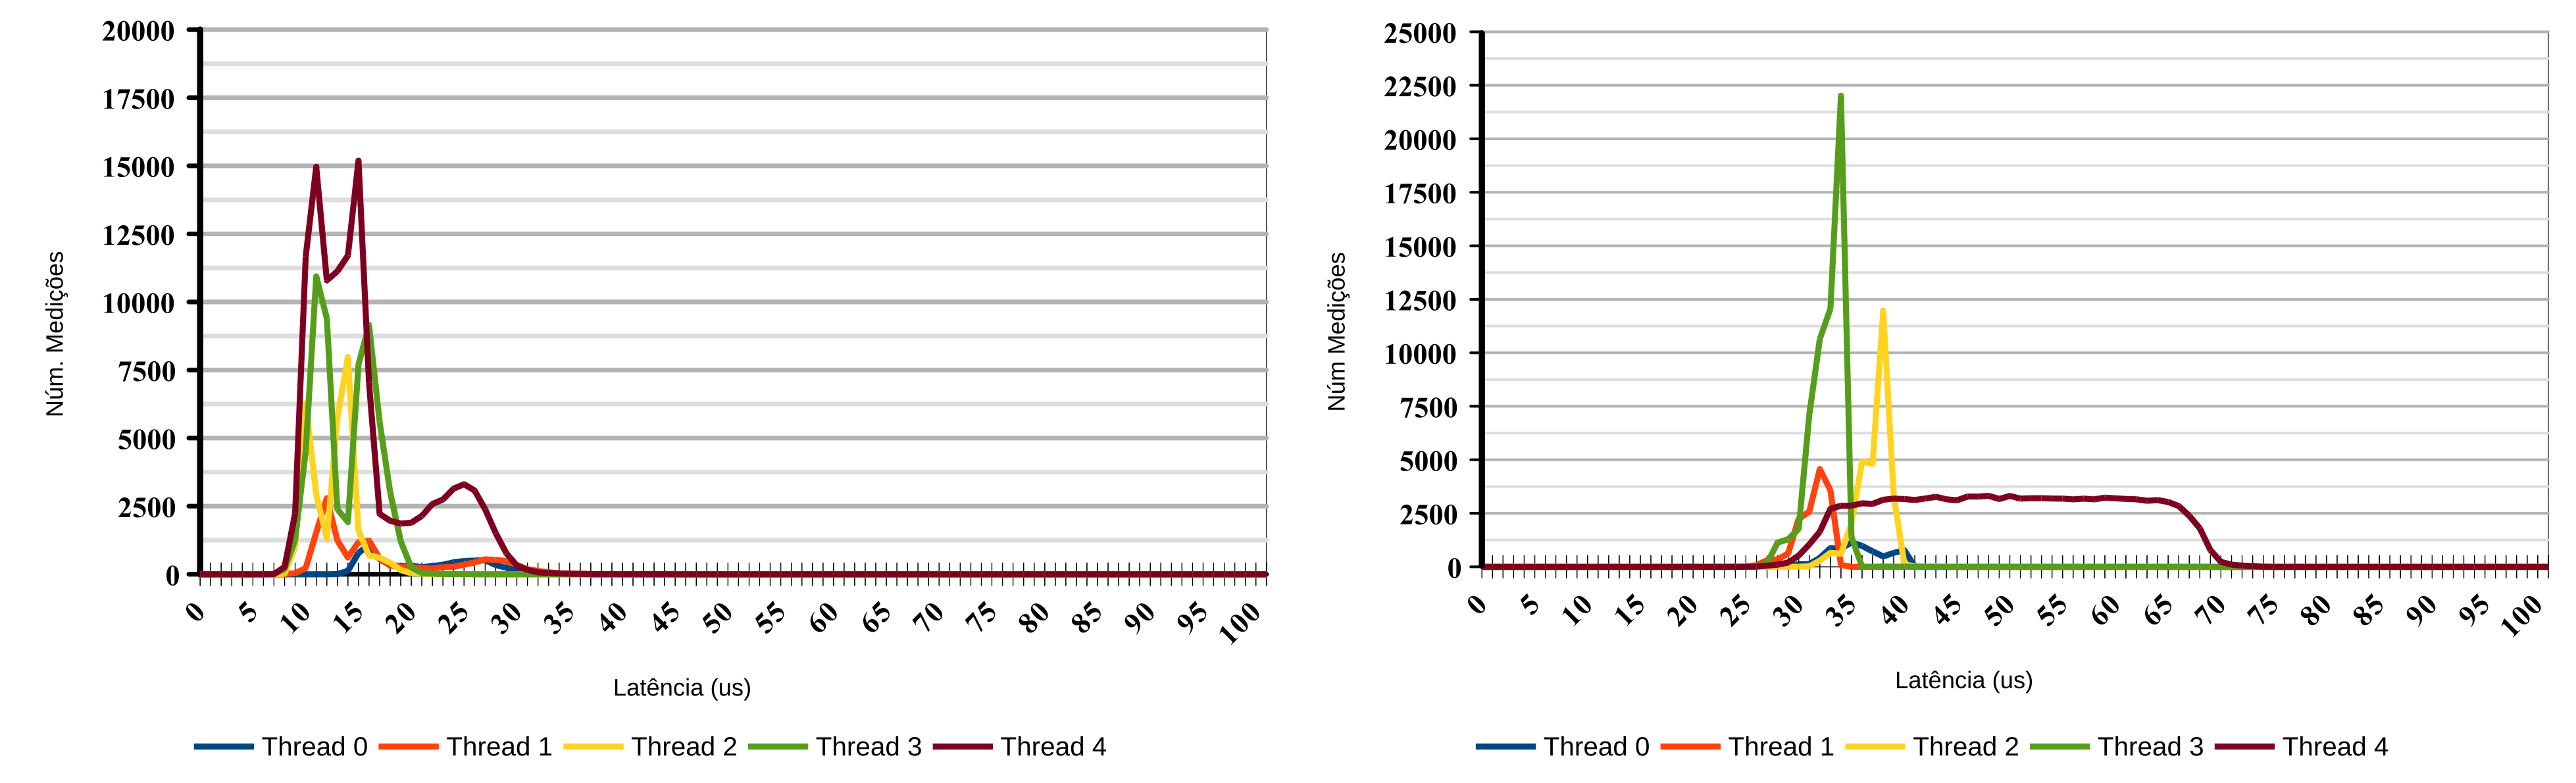
\includegraphics{serie-phPRTvsRTAI}
    \caption{Medidas de latência dos testes \textit{Serie-PH} - Preempt\_RT x RTAI}
    \label{serie-phPRTvsRTAI}
\end{figure}

\begin{figure}[!htb]
    \centering
    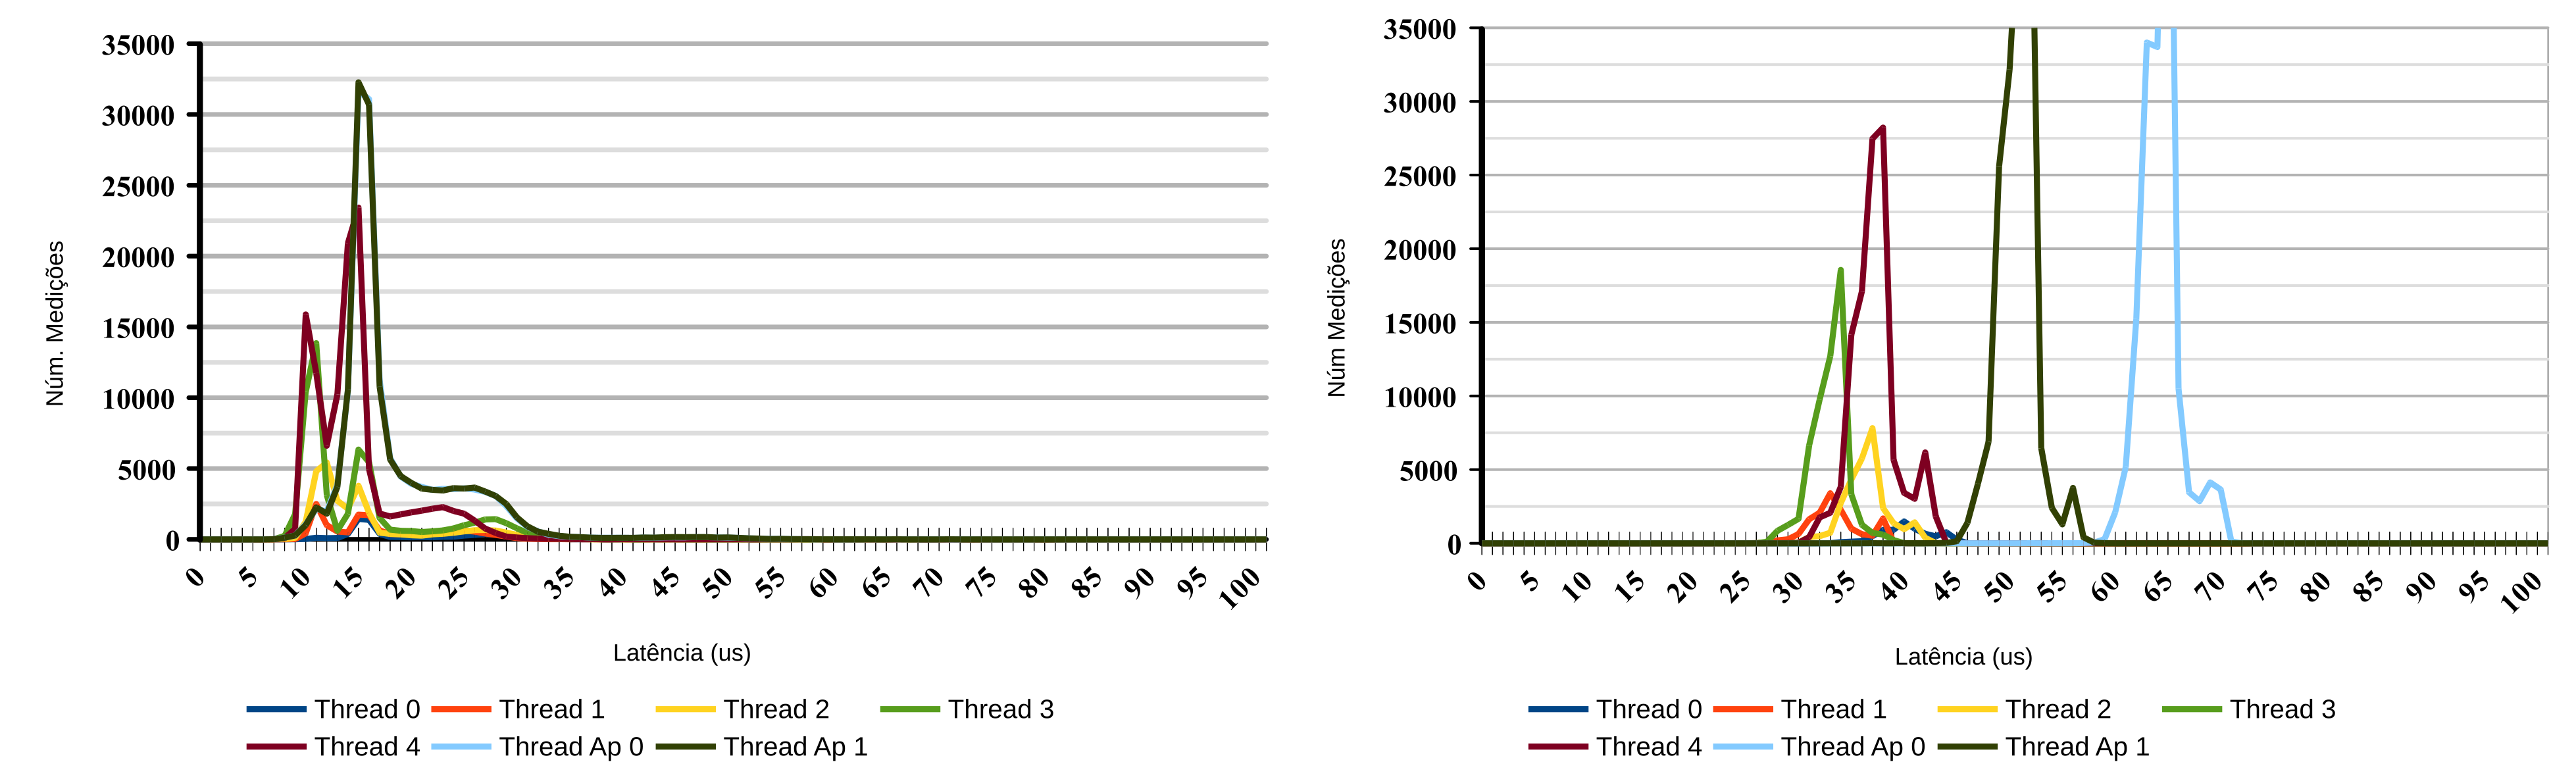
\includegraphics{serie-ahPRTvsRTAI}
    \caption{Medidas de latência dos testes \textit{Serie-AH} - Preempt\_RT x RTAI}
    \label{serie-ahPRTvsRTAI}
\end{figure}

\begin{table}
\begin{tabular}{c|c|c|c|c|}
\cline{2-5} 
 & \multicolumn{2}{c|}{Preempt\_RT} & \multicolumn{2}{c|}{RTAI} \\ 
\hline 
\multicolumn{1}{ |c| }{\textit{Thread}} & Latência Máx. & Latência Mín & Latência Máx. & Latência Mín \\ 
\hline 
\multicolumn{1}{ |c| }{0} & 39 & 13 & 41 & 28 \\ 
\hline 
\multicolumn{1}{ |c| }{1} & 43 & 8 & 38 & 22 \\ 
\hline 
\multicolumn{1}{ |c| }{2} & 30 & 8 & 44 & 27 \\ 
\hline 
\multicolumn{1}{ |c| }{3} & 25 & 7 & 40 & 24 \\ 
\hline 
\multicolumn{1}{ |c| }{4} & 44 & 7 & 74 & 20 \\ 
\hline 
\end{tabular} 
\caption{Valores (em \si{\micro\s}) máximos e mínimos de latência obtidos nos testes \textit{Serie-PH}- Preempt\_RT x RTAI}
\label{serie-phTabela}
\end{table}

\begin{table}
\begin{tabular}{c|c|c|c|c|}
\cline{2-5} 
 & \multicolumn{2}{c|}{Preempt\_RT} & \multicolumn{2}{c|}{RTAI} \\ 
\hline 
\multicolumn{1}{ |c| }{\textit{Thread}} & Latência Máx. & Latência Mín & Latência Máx. & Latência Mín \\ 
\hline 
\multicolumn{1}{ |c| }{0} & 70 & 9 & 46 & 32 \\ 
\hline 
\multicolumn{1}{ |c| }{1} & 72 & 8 & 39 & 25 \\ 
\hline 
\multicolumn{1}{ |c| }{2} & 71 & 7 & 43 & 28 \\ 
\hline 
\multicolumn{1}{ |c| }{3} & 74 & 7 & 39 & 21 \\ 
\hline 
\multicolumn{1}{ |c| }{4} & 67 & 7 & 45 & 23 \\ 
\hline 
\multicolumn{1}{ |c| }{Ap. 0} & 80 & 6 & 72 & 52 \\ 
\hline 
\multicolumn{1}{ |c| }{Ap. 1} & 71 & 7 & 59 & 37 \\ 
\hline 
\end{tabular} 
\caption{Valores (em \si{\micro\s}) máximos e mínimos de latência obtidos nos testes \textit{Serie-AH}- Preempt\_RT x RTAI}
\label{serie-ahTabela}
\end{table}

\begin{table}
\begin{tabular}{c|c|c|c|c|}
\cline{2-5} 
 & \multicolumn{2}{c|}{Preempt\_RT} & \multicolumn{2}{c|}{RTAI} \\ 
\hline 
\multicolumn{1}{ |c| }{\textit{Thread}} & Tc (\textit{Serie-PH}). & Tc (\textit{Serie-AH}) & Tc (\textit{Serie-PH}) & Tc (\textit{Serie-AH}) \\ 
\hline 
\multicolumn{1}{ |c| }{0} & 18 & 70 & 19 & 21 \\ 
\hline 
\multicolumn{1}{ |c| }{1} & 38 & 81 & 45 & 45 \\ 
\hline 
\multicolumn{1}{ |c| }{2} & 39 & 83 & 37 & 36 \\ 
\hline 
\multicolumn{1}{ |c| }{3} & 27 & 70 & 28 & 20 \\ 
\hline 
\multicolumn{1}{ |c| }{4} & 39 & 79 & 43 & 40 \\ 
\hline 
\multicolumn{1}{ |c| }{Ap. 0} & - & 62 & - & 42 \\ 
\hline 
\multicolumn{1}{ |c| }{Ap. 1} & - & 56 & - & 44 \\ 
\hline 
\end{tabular} 
\caption{Valores (em \si{\micro\s}) do tempo de computação máximo obtidos nos testes \textit{Serie-PH} e \textit{Serie-AH} - Preempt\_RT x RTAI}
\label{serie-ahTabela}
\end{table}
